\documentclass[11pt]{article}
\usepackage{graphicx}
\usepackage{hyperref}
%\usepackage{appendix}
\usepackage{amsmath}
\usepackage{amsthm}
\usepackage{amssymb}
\usepackage{float}
\usepackage{commath}
\usepackage{booktabs}
\renewcommand{\arraystretch}{1.2}
\usepackage{siunitx}
\sisetup{detect-all}
\usepackage{listings}
\usepackage{color} %red, green, blue, yellow, cyan, magenta, black, white
\definecolor{mygreen}{RGB}{28,172,0} % color values Red, Green, Blue
\definecolor{mylilas}{RGB}{170,55,241}
\usepackage[a4paper,margin=20mm]{geometry}
\numberwithin{equation}{section}
\setlength{\parskip}{\baselineskip}
\setlength{\parindent}{0pt}
\hypersetup{
    colorlinks=true,
    linkcolor=black,
    filecolor=black,      
    urlcolor=black,
    citecolor=black
}
\urlstyle{same}
\begin{document}
\title{\textbf{UCL Mechanical Engineering 2020/2021}\\ENGF0004 48-hour Project}
\author{NCWT3}
\maketitle
\tableofcontents
\listoffigures
\section{PDEs, Matrix applications}
\section{Vector calculus}
\section{Transforms}
\subsection{Plot of data}
\lstset{language=Matlab,%
    %basicstyle=\color{red},
    breaklines=true,%
    morekeywords={matlab2tikz},
    keywordstyle=\color{blue},%
    morekeywords=[2]{1}, keywordstyle=[2]{\color{black}},
    identifierstyle=\color{black},%
    stringstyle=\color{mylilas},
    commentstyle=\color{mygreen},%
    showstringspaces=false,%without this there will be a symbol in the places where there is a space
    numbers=left,%
    numberstyle={\tiny \color{black}},% size of the numbers
    numbersep=9pt, % this defines how far the numbers are from the text
    emph=[1]{for,end,break},emphstyle=[1]\color{red}, %some words to emphasise
    %emph=[2]{word1,word2}, emphstyle=[2]{style},    
}
\lstinputlisting{./mCode/q301a.m}
\begin{figure}[H]
    \centering
    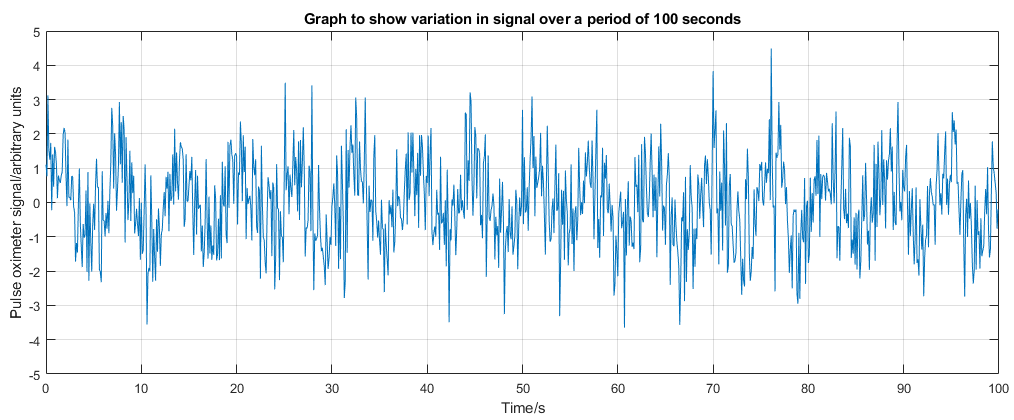
\includegraphics[width = \textwidth]{./img/q301a.png}
    \caption{Graph to show variation in signal over a period of 100 seconds.}
\end{figure}
\subsection{Plot of Fourier transform}
\lstset{language=Matlab,%
    %basicstyle=\color{red},
    breaklines=true,%
    morekeywords={matlab2tikz},
    keywordstyle=\color{blue},%
    morekeywords=[2]{1}, keywordstyle=[2]{\color{black}},
    identifierstyle=\color{black},%
    stringstyle=\color{mylilas},
    commentstyle=\color{mygreen},%
    showstringspaces=false,%without this there will be a symbol in the places where there is a space
    numbers=left,%
    numberstyle={\tiny \color{black}},% size of the numbers
    numbersep=9pt, % this defines how far the numbers are from the text
    emph=[1]{for,end,break},emphstyle=[1]\color{red}, %some words to emphasise
    %emph=[2]{word1,word2}, emphstyle=[2]{style},    
}
\lstinputlisting{./mCode/q302a.m}
\begin{figure}[H]
    \centering
    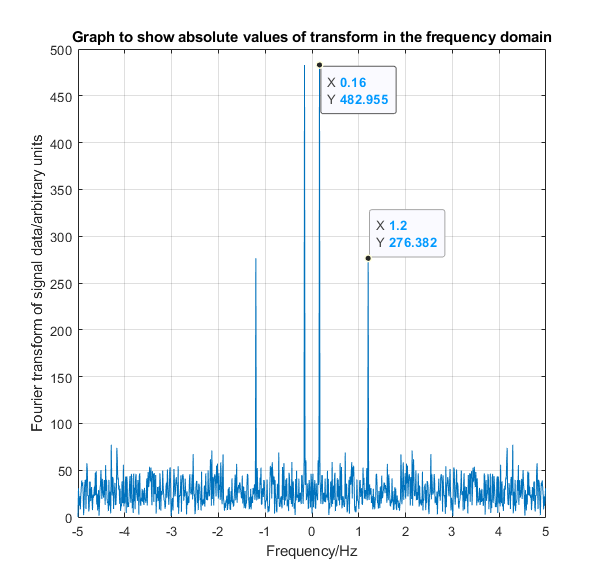
\includegraphics[height = 10cm]{./img/q302a.png}
    \caption{Graph to show absolute values of transform in the frequency domain.}
    \label{fig:q302a}
\end{figure}
\subsection{Extraction of patient's cardiac and respiratory cycle}
As seen from Figure \ref{fig:q302a}, we can extract two values from our Fourier transform. The higher peak has a frequency of \SI{0.16}{\hertz} and a period of \SI{6.25}{\second}. This represents the breathing of the subject (9.6 breaths per minute). According to a Cleveland Clinic article on vital signs, the average human breathing rate for adults should be around 12-16 breaths per minute \cite{q3.3.1}. The lower peak has a frequency of \SI{1.2}{\hertz} and a period of \SI{0.83}{\second}. This represents the heartbeat of the subject (72 beats per minute). According to the British Heart Foundation, the average resting heart rate for adults is between 60-100 beats per minute \cite{q3.3.2}.
\subsection{Frequency filter}
\subsubsection{Gaussian functions}
A Gaussian function was generated using MATLAB's "normpdf" function. $\mu = \pm1.2$. The value for $\sigma$ was selected arbitrarily to de-noise the signal to an appropriate level
\lstset{language=Matlab,%
    %basicstyle=\color{red},
    breaklines=true,%
    morekeywords={matlab2tikz},
    keywordstyle=\color{blue},%
    morekeywords=[2]{1}, keywordstyle=[2]{\color{black}},
    identifierstyle=\color{black},%
    stringstyle=\color{mylilas},
    commentstyle=\color{mygreen},%
    showstringspaces=false,%without this there will be a symbol in the places where there is a space
    numbers=left,%
    numberstyle={\tiny \color{black}},% size of the numbers
    numbersep=9pt, % this defines how far the numbers are from the text
    emph=[1]{for,end,break},emphstyle=[1]\color{red}, %some words to emphasise
    %emph=[2]{word1,word2}, emphstyle=[2]{style},    
}
\lstinputlisting{./mCode/q304a.m}
\begin{figure}[H]
    \centering
    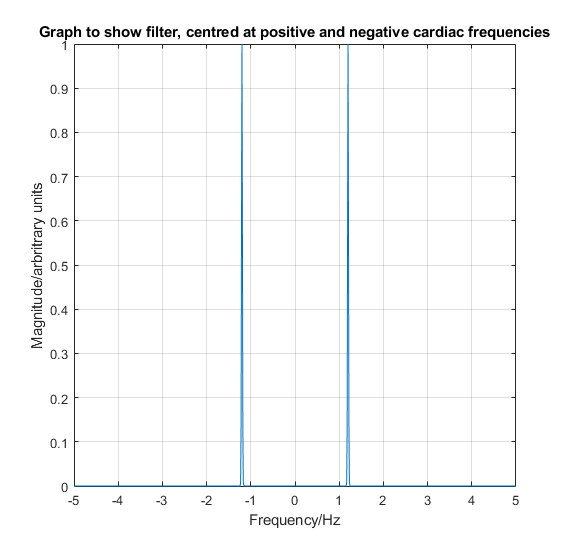
\includegraphics[height = 10cm]{./img/q304a.png}
    \caption{Graph to show filter, centred at positive and negative cardiac frequencies.}
    \label{fig:q304a}
\end{figure}
\subsubsection{Filtered/unfiltered Fourier data comparison}
\lstset{language=Matlab,%
    %basicstyle=\color{red},
    breaklines=true,%
    morekeywords={matlab2tikz},
    keywordstyle=\color{blue},%
    morekeywords=[2]{1}, keywordstyle=[2]{\color{black}},
    identifierstyle=\color{black},%
    stringstyle=\color{mylilas},
    commentstyle=\color{mygreen},%
    showstringspaces=false,%without this there will be a symbol in the places where there is a space
    numbers=left,%
    numberstyle={\tiny \color{black}},% size of the numbers
    numbersep=9pt, % this defines how far the numbers are from the text
    emph=[1]{for,end,break},emphstyle=[1]\color{red}, %some words to emphasise
    %emph=[2]{word1,word2}, emphstyle=[2]{style},    
}
\lstinputlisting{./mCode/q304b.m}
\begin{figure}[H]
    \centering
    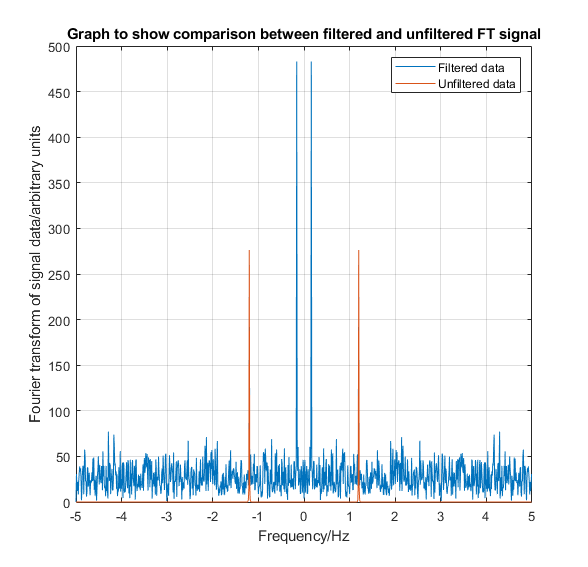
\includegraphics[height = 9cm]{./img/q304b.png}
    \caption{Graph to show comparison between filtered and unfiltered FT signal.}
    \label{fig:q304b}
\end{figure}
\begin{figure}[H]
    \centering
    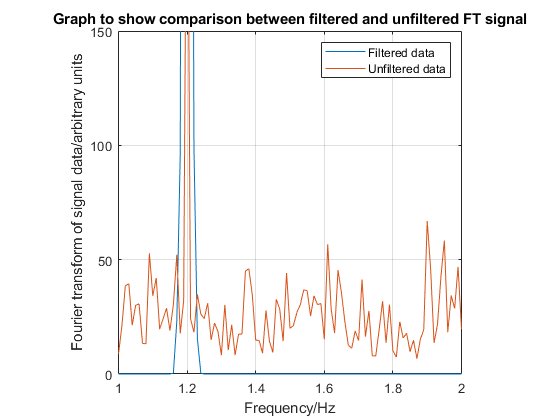
\includegraphics[height = 9cm]{./img/q304b2.png}
    \caption{Graph to show comparison between filtered and unfiltered FT signal (close-up).}
    \label{fig:q304b}
\end{figure}
\subsection{Filtered data}
\lstset{language=Matlab,%
    %basicstyle=\color{red},
    breaklines=true,%
    morekeywords={matlab2tikz},
    keywordstyle=\color{blue},%
    morekeywords=[2]{1}, keywordstyle=[2]{\color{black}},
    identifierstyle=\color{black},%
    stringstyle=\color{mylilas},
    commentstyle=\color{mygreen},%
    showstringspaces=false,%without this there will be a symbol in the places where there is a space
    numbers=left,%
    numberstyle={\tiny \color{black}},% size of the numbers
    numbersep=9pt, % this defines how far the numbers are from the text
    emph=[1]{for,end,break},emphstyle=[1]\color{red}, %some words to emphasise
    %emph=[2]{word1,word2}, emphstyle=[2]{style},    
}
\lstinputlisting{./mCode/q305a.m}
\begin{figure}[H]
    \centering
    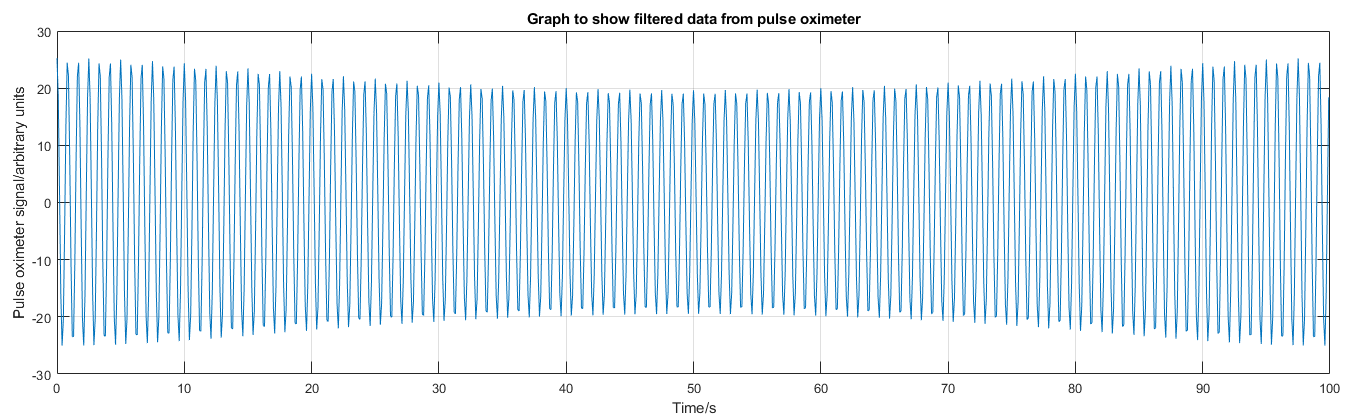
\includegraphics[width = \textwidth]{./img/q305a.png}
    \caption{Graph to show filtered data from pulse oximeter.}
    \label{fig:q305a}
\end{figure}
\subsection{Effect of varying the width of Gaussian function}
The code was adjusted to created two additional cases, to make four in total:
\begin{itemize}
    \item Unfiltered data
    \item Gaussian filter with $\sigma = 0.1$
    \item Gaussian filter with $\sigma = 0.01$
    \item Gaussian filter with $\sigma = 0.001$
\end{itemize}
\lstset{language=Matlab,%
    %basicstyle=\color{red},
    breaklines=true,%
    morekeywords={matlab2tikz},
    keywordstyle=\color{blue},%
    morekeywords=[2]{1}, keywordstyle=[2]{\color{black}},
    identifierstyle=\color{black},%
    stringstyle=\color{mylilas},
    commentstyle=\color{mygreen},%
    showstringspaces=false,%without this there will be a symbol in the places where there is a space
    numbers=left,%
    numberstyle={\tiny \color{black}},% size of the numbers
    numbersep=9pt, % this defines how far the numbers are from the text
    emph=[1]{for,end,break},emphstyle=[1]\color{red}, %some words to emphasise
    %emph=[2]{word1,word2}, emphstyle=[2]{style},    
}
\lstinputlisting{./mCode/q306a.m}
\begin{figure}[H]
    \centering
    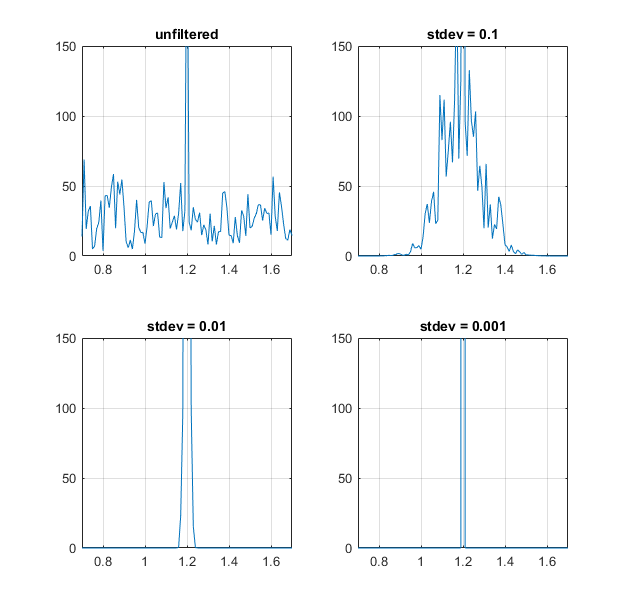
\includegraphics[width = \textwidth]{./img/q306a.png}
    \caption{Graphs to compare the effect of varying Gaussian filter width on FT signal.}
    \label{fig:q306a}
\end{figure}
Here we can see that adjusting the value of $\sigma$ effects the amount of noise that appears at the base of the peak in the Fourier transformed data. For $\sigma = 0.1$, there is still quite a bit of residual noise. $\sigma = 0.01$ and $\sigma = 0.001$ both do not exhibit any noise at the base, but we can see that for $\sigma = 0.01$, there is a slight flaring at the base.
\begin{figure}[H]
    \centering
    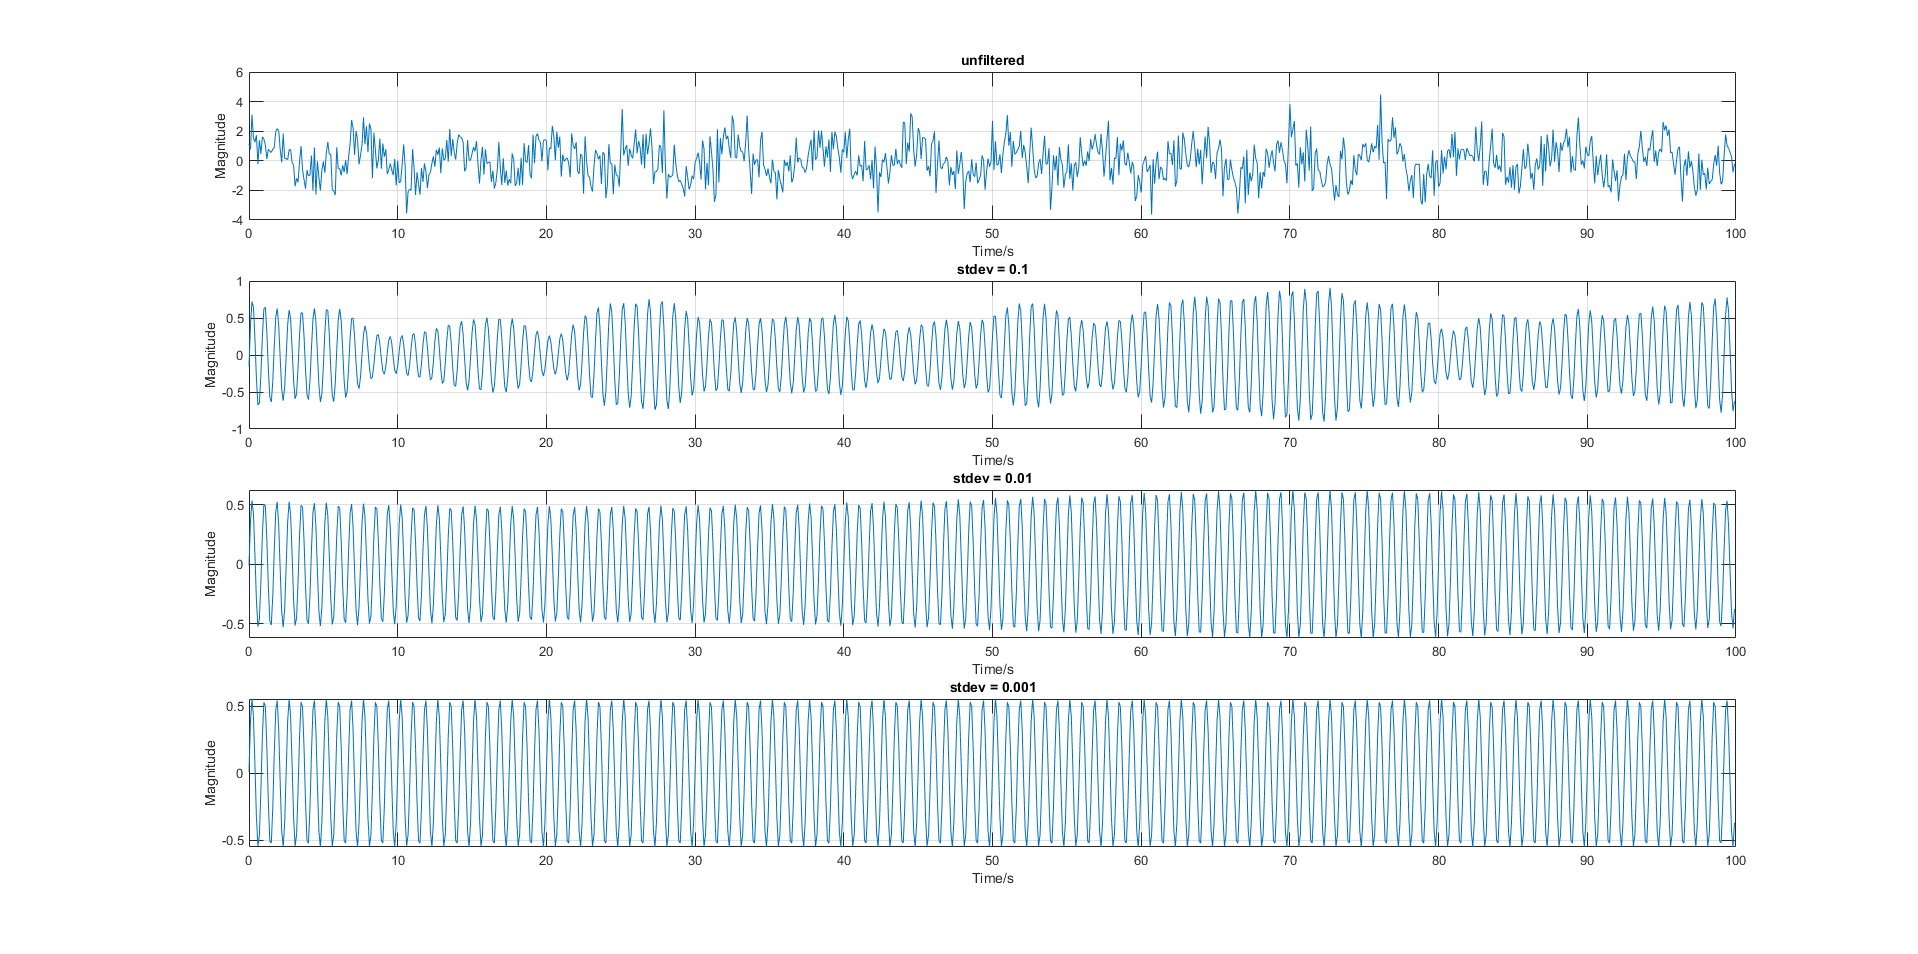
\includegraphics[width = \textwidth]{./img/q306b.png}
    \caption{Graphs to compare the effect of varying Gaussian filter width on signal from pulse oximeter.}
    \label{fig:q306b}
\end{figure}
Here we can see the effect of the residual noise in the $\sigma = 0.1$ case, with relatively large variations in the amplitude of the signal. We can also see the effect of the flared base in the $\sigma = 0.01$ case as a smooth decrease and then increase in the amplitude of the signal. The $\sigma = 0.001$ case represents a virtually perfect signal with a frequency of \SI{1.2}{\hertz}.
\begin{thebibliography}{00}
    \bibitem{q3.3.1} Cleveland Clinic, "Vital Signs", \url{https://www.hopkinsmedicine.org/health/conditions-and-diseases/vital-signs-body-temperature-pulse-rate-respiration-rate-blood-pressure#:~:text=Respiration%20rates%20may%20increase%20with,to%2016%20breaths%20per%20minute.} Accessed 27/04/21 14:47
    \bibitem{q3.3.2} British Heart Foundation, "What is a normal pulse rate?", \url{https://www.bhf.org.uk/informationsupport/heart-matters-magazine/medical/ask-the-experts/pulse-rate#:~:text=A%20normal%20resting%20heart%20rate,rich%20blood%20around%20the%20body.} Accessed 27/04/21 14:45
\end{thebibliography}
\end{document}